\documentclass{zc-ust-hw}

\usepackage{lipsum}

\name{SalahDin Ahmed Salh Rezk}
\id{202201079}
\course{Thermo, Wave Motion and Optics (PHYS 201)}
\assignment{Participation 4}

\begin{document}

\maketitle

In the lecture, we solved the problem of the interfence of light for the double
slits experiment, using the superposition prinicple. Now suppose a
configuration of three slits as shown in the figure below.

\begin{figure}[htpb]
  \begin{center}
    \includegraphics[width=0.3\textwidth]{figures/1705951832.png}
  \end{center}
  \caption{}
\end{figure}


\begin{enumerate}
  \item Using the same procedures we adapted, deduce that the total intensity
    of light recivied at the screen in such a case as function of \(\theta\) takes the
    following form:
    \[
      I=\frac{I_{0}}{9}\left[ 1+2\cos \left(\frac{2\pi d\sin \theta }{\lambda }\right)\right]^2
    .\] 
    \begin{sol}
      \begin{align}
        E_{1}&= E_{0}\sin (\omega t) \\
        E_{2}&= E_{0}\sin (\omega t+\phi ) \\
        E_{3}&= E_{0}\sin (\omega t+2\phi ) \\
        \phi &= \frac{2\pi d}{\lambda }\sin \theta \\
        \intertext{From phasor diagram:}
        E &= E_{0} (1+2\cos \phi ) \\
        I &\propto E^2 \\
        I &= kE^2 \\
          &= k \left[ E_{0} (1+2\cos \phi ) \right]^2 \\
          \intertext{For \( \phi =0 \):}
        I_{0} &= 9kE_{0}^2 \implies k = \frac{I_{0}}{9E_{0}^2} \\
        I&=\frac{I_{0}}{9}\left[ 1+2\cos \left(\frac{2\pi d\sin \theta }{\lambda }\right)\right]^2
      \end{align}
    \end{sol}
  \item To understand what this implies, plot \( I / I_{0} \) versus \( d\sin \theta /\lambda\).
    
    \begin{figure}[htpb]
    \centering
    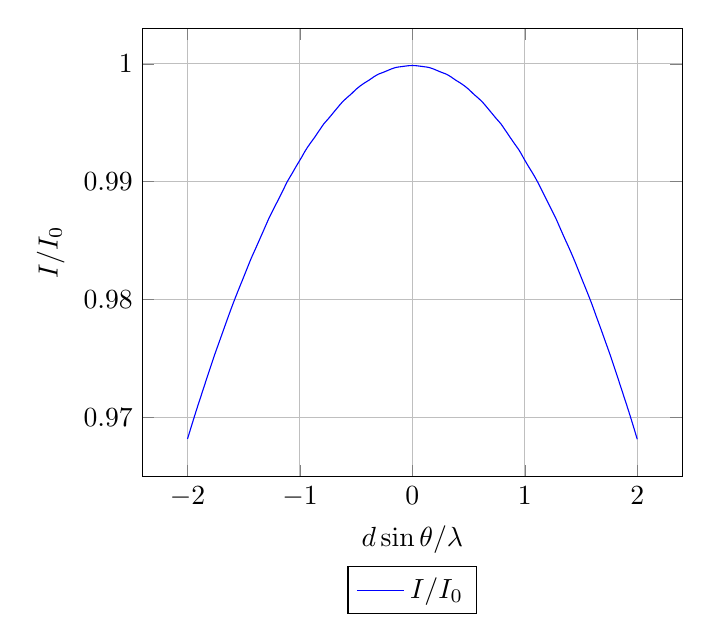
\begin{tikzpicture}
        \begin{axis}[
            xlabel={$d\sin\theta/\lambda$},
            ylabel={$I/I_0$},
            domain=-2:2,
            samples=100,
            grid=major,
            legend style={at={(0.5,-0.2)},anchor=north},
        ]
        
        % Parameters
        \pgfmathsetmacro{\Izero}{1}  % Set the value of I_0
        \pgfmathsetmacro{\lambdaValue}{1}  % Set the value of lambda
        
        % Plot the function
        \addplot[blue,smooth] {(\Izero/9)*(1 + 2*cos(2*pi*x/\lambdaValue))^2};
        \addlegendentry{$I/I_0$};
        
        \end{axis}
    \end{tikzpicture}
\end{figure}

\end{enumerate}

\end{document}
